\documentclass[a4paper,12pt]{report}
\usepackage{a4wide}

%\documentclass[a5paper,10pt]{book}
%\usepackage[top=23mm, bottom=18mm, left=15mm, right=25mm]{geometry}
%\geometry{papersize={170mm,220mm}}


\usepackage[utf8x]{inputenc}
\usepackage[danish]{babel}

\usepackage{xr-hyper} %Externe hyper-ref
\usepackage[colorlinks=true, hyperindex=true, linkcolor=minmblaa, citecolor=minmblaa, urlcolor=minmblaa]{hyperref}
\hypersetup{colorlinks=true,filecolor=minmblaa,bookmarksnumbered=true} %Til hyperreferencer. Referencer med farver
\usepackage{needspace} % giver mulighed for at kræve at der skal være et antal tomme linier på siden før ellers indsættes et sideskift.
\usepackage{framed} %Bokse
\usepackage{wrapfig}

\usepackage{amsmath,amsfonts,amssymb,amsthm,mathtools} %Matematikpakker

\setlength{\parindent}{0mm} %Ingen Indhak i første linje i afsnit

\usepackage{color} %Farvepakke

\usepackage{array}
\usepackage{colortbl}
\usepackage{multirow} %Til at flette rækker i tabeller.

\usepackage{verbatim,mhchem}



	% DOWNLOAD FRA: http://sarovar.org/frs/?group_id=52&release_id=97
	% Læg i directory for hoved TEX fil
%\usepackage[draft]{pdfdraftcopy}
%\draftstring{Licens: Kasper Langt Mellemnavn Skårhøj}
%\draftfontsize{30}
	%\draftfontfamily{hlh}
	%\draftangle{45}
	%\definecolor{mycolor}{rgb}{.825,.855,1}
	%\draftcolor{mycolor}
	%\draftfontattrib



% = Sidehoved =
\usepackage{fancyhdr}
\pagestyle{fancy}
\renewcommand{\sectionmark}[1]{\markright{\protect\titlegraphic{dturoed}\textcolor{dtugraa}{\thesection~\MakeUppercase{#1}}}} % \thesection.\
\fancyhead{}
\fancyfoot{}
\fancyhead[R]{\titlefont\thepage}
\fancyhead[C]{}
\fancyhead[L]{\titlefont \small eNote \MakeUppercase{~\thechapter}~\hspace*{1ex}\rightmark}
\renewcommand\headrulewidth{0pt}
\fancypagestyle{plain}{\fancyfoot[C]{}}% {\titlefont\footnotesize\thepage}}
\setlength{\headheight}{15pt}


% = Længder
%\newlength{\envtblsep}\setlength{\envtblsep}{1\FrameSep}
\newlength{\obsl}\setlength{\obsl}{\textwidth-1.2cm-13.2pt}

% Includes:

% =     Fonts (select one)    =
\usepackage{mathpazo}\linespread{1.05} % Palatino needs more leading (space between lines)
\usepackage{bm} % bold math, must be loaded after the fontpackages

% % Til overskrifter
\DeclareTextFontCommand{\th}{\fontencoding{T1}\fontfamily{phv}\fontseries{b}\selectfont}
\newcommand\titlefont{\fontencoding{T1}\fontfamily{phv}\selectfont}


% =     PGF grafik      =
\usepackage{tikz}
\newcommand\titlegraphic[1]{%
\tikz[baseline] %
\draw[thick,color=#1]
(0pt  ,-0.25em) -- (0pt  ,0.85em)
(2.5pt,-0.25em) -- (2.5pt,0.85em)
(5pt  ,-0.25em) -- (5pt  ,0.85em)
(7.5pt,-0.25em) -- (7.5pt,0.85em);\hspace*{0.8ex} %
}

\newcommand\titlegraphicwide[1]{%
\tikz[baseline] %
\draw[line width=0.8mm,color=#1]
(0pt  ,-0.25em) -- (0pt  ,0.85em)
(4.5pt,-0.25em) -- (4.5pt,0.85em)
(9pt  ,-0.25em) -- (9pt  ,0.85em)
(13.5pt,-0.25em) -- (13.5pt,0.85em);\hspace*{0.8ex} %
}


% =      Title Layout      =
\usepackage{titlesec}
\makeatletter
\titleformat{\chapter}
	[display] % Shape
	{\titlefont\Huge\flushleft} % Title and label format
	{\titlefont\LARGE\bfseries \titlegraphicwide{dturoed}\textcolor{dtugraa}{\@chapapp~\thechapter}} % label
	{0.9em} % label/title separation
	{} % before code
	[] % after code
\makeatother
\titleformat{\section}
	[hang] % Shape
	{\titlefont\Large\flushleft} % Title and label format
	{\thesection} % label
	{0.9em} % label/title separation
	{} % before code
	[] % after code
\titleformat{\subsection}
	[hang] % Shape
	{\titlefont\large} % Title and label format
	{\thesubsection} % label
	{0.9em} % label/title separation
	{} % before code
	[] % after code
\titlespacing{\subsection}{0pt}{*6}{*1.5}
\titleformat{\subsubsection}
	[hang] % Shape
	{\titlefont} % Title and label format
	{\thesubsubsection} % label
	{0.9em} % label/title separation
	{} % before code
	[] % after code



% = Farver
\definecolor{dturoed}{rgb}{0.6, 0.0, 0.0}
\definecolor{dtugraa}{rgb}{0.5, 0.5, 0.5}	% Lidt mørkere. Korrekt = 0.4
\definecolor{mingroenstreg}{rgb}{0.4,0.8,0}	% Sekundærfarve 14 : 102/204/0	(Forårsgrøn) -> Eksempler
\definecolor{mingroen}{rgb}{0.32,0.64,0}		% Sekundærfarve 14, 80% mørkere (tekst)
\definecolor{minorangestreg}{rgb}{1,0.6,0}		% Sekundærfarve 1 : 255/153/0	(Orange) -> Opgaver
\definecolor{minorange}{rgb}{0.8,0.48,0}		% Sekundærfarve 1 , 80% mørkere (tekst)

\definecolor{minblaa}{rgb}{0.2,0.4,0.8}	% Sekundærfarve 13 , 51/102/204 	( Blå -> Definitioner etc)
\definecolor{minmblaa}{rgb}{0.16,0.32,0.64}	% Sekundærfarve 13 , 80% mørkere (tekst)
\definecolor{thmbackground}{rgb}{0.97,.97, 0.99}	% Farve 13 - lys baggrund

\definecolor{mingraastreg}{rgb}{.5,.5,.5}
\definecolor{hvadbackground}{rgb}{0.97,.97, 0.97}
\definecolor{sumgul}{rgb}{1,1,.8}

\definecolor{hjmopgfarve}{rgb}{.96,1,.96}


% = Counter
\newcounter{evncount}[chapter]
\setcounter{evncount}{0}
\renewcommand{\theevncount}{\thechapter.\arabic{evncount}}
\renewcommand{\theequation}{\thechapter-\arabic{equation}}


% = Eksempler = example =
\newenvironment{example}[1][]{
	\refstepcounter{evncount}
	\setlength{\obsl}{\textwidth-1.2cm-13.2pt-9pt} % fix width of the info envirnment%
	\def\FrameCommand{ 
		\textcolor{mingroenstreg}{\vrule width 4pt} 
		\hspace{5pt} 
	}%
	\MakeFramed{\advance\hsize-\width \FrameRestore}%
	\needspace{3\baselineskip}
	\titlegraphic{mingroen}
	\textcolor{mingroen}{
		\th{Eksempel \theevncount \hspace*{5mm} #1}
	} 
	\vspace*{3mm}%
	\begin{small}
	\par
}
{
	\end{small}
	\endMakeFramed
}


% = Opgaver = exercise =
\newenvironment{exercise}[1][]{
	\refstepcounter{evncount}
	\setlength{\obsl}{\textwidth-1.2cm-13.2pt-9pt}% fix width of the info envirnment%
	\def\FrameCommand{
		\textcolor{minorangestreg}{\vrule width 4pt}
		\hspace{5pt}
	}%
	\MakeFramed{\advance\hsize-\width \FrameRestore}%
	\needspace{3\baselineskip}
	\titlegraphic{minorange}
	\textcolor{minorange}{
		\th{Opgave \theevncount \hspace*{5mm} #1}
	} 
	\vspace*{3mm}%
	\begin{small}
	\par
}
{
	\end{small}
	\endMakeFramed
}


% = Bevis
\newenvironment{bevis}{
	\setlength{\obsl}{\textwidth-1.2cm-13.2pt-9pt} % fix width of the info envirnment%
	\def\FrameCommand{
		\textcolor{mingraastreg}{\vrule width 4pt} 
		\hspace{5pt}
	}%
	\MakeFramed{\advance\hsize-\width \FrameRestore}%
	\needspace{3\baselineskip}
	\titlegraphic{black}
	\textcolor{black}{
		\th{Bevis}
	}
	\vspace*{3mm}%
	\begin{small}
	\par
}
{
	\bevisslut 
	\end{small}
	\endMakeFramed
}


% = Definition =
\newenvironment{definition}[1][]{
	\vspace{4mm}
	\pagebreak[1]
	\setlength{\obsl}{\textwidth-1.2cm-2\FrameSep-13.2pt}%
	\def\FrameCommand{
		\fboxsep=\FrameSep\fcolorbox{minblaa}{thmbackground}
	}
	\begin{minipage}{\textwidth}
	\MakeFramed{\advance\hsize-\width\FrameRestore}
	\refstepcounter{evncount}
	\titlegraphic{minblaa}
	\textcolor{minmblaa}{
		\th{Definition \theevncount \hspace*{5mm} #1}
	}
	\vspace*{3mm}
	\par
}
{
	\endMakeFramed 
	\end{minipage}
	\vspace{4mm}
}


% = Theorem =
\newenvironment{theorem}[1][]{
	\vspace{4mm}
	\pagebreak[1]%
	\setlength{\obsl}{\textwidth-1.2cm-2\FrameSep-13.2pt}%
	\def\FrameCommand{
		\fboxsep=\FrameSep\fcolorbox{minblaa}{thmbackground}
	}%
	\begin{minipage}{\textwidth}
	\MakeFramed{\advance\hsize-\width\FrameRestore}%
	\refstepcounter{evncount}
	\titlegraphic{minblaa}
	\textcolor{minmblaa}{
		\th{Sætning \theevncount \hspace*{5mm} #1}
	}
	\vspace*{3mm}
	\par
}
{
	\endMakeFramed 
	\end{minipage}
	\vspace{4mm}
}


% = Lemma =
\newenvironment{lemma}[1][]{
	\vspace{4mm}
	\pagebreak[1]
	\setlength{\obsl}{\textwidth-1.2cm-2\FrameSep-13.2pt}%
	\def\FrameCommand{
		\fboxsep=\FrameSep \fcolorbox{minblaa}{thmbackground}
	}
	\begin{minipage}{\textwidth} 
	\MakeFramed{\advance\hsize-\width \FrameRestore}
	\refstepcounter{evncount}
	\titlegraphic{minblaa}
	\textcolor{minmblaa}{
		\th{Hjælpesætning \theevncount \hspace*{5mm} #1}
	}
	\vspace*{3mm}
	\par
}
{
	\endMakeFramed 
	\end{minipage}
	\vspace{4mm}
}


% = Corollary =
\newenvironment{corollary}[1][]{
	\vspace{4mm}
	\pagebreak[1]
	\setlength{\obsl}{\textwidth-1.2cm-2\FrameSep-13.2pt}%
	\def\FrameCommand{
		\fboxsep=\FrameSep \fcolorbox{minblaa}{thmbackground}
	}
	\begin{minipage}{\textwidth} 
	\MakeFramed{\advance\hsize-\width \FrameRestore}
	\refstepcounter{evncount}
	\titlegraphic{minblaa}
	\textcolor{minmblaa}{
		\th{Følgesætning \theevncount \hspace*{5mm} #1}
	}
	\vspace*{3mm}
	\par
}
{
	\endMakeFramed 
	\end{minipage}
	\vspace{4mm}
}


% = Metode = method
\newenvironment{method}[1][]{
	\vspace{4mm}
	\pagebreak[1]
	\setlength{\obsl}{\textwidth-1.2cm-2\FrameSep-13.2pt}%
	\def\FrameCommand{
		\fboxsep=\FrameSep \fcolorbox{black}{hvadbackground}
	}
	\begin{minipage}{\textwidth} 
	\MakeFramed{\advance\hsize-\width \FrameRestore}
	\refstepcounter{evncount}
	\titlegraphic{black}
	\textcolor{black}{
		\th{Metode \theevncount \hspace*{5mm} #1}
	}
	\vspace*{3mm}
	\par
}
{
	\endMakeFramed
	\end{minipage}
	\vspace{4mm}
}


% = Forklaring = explain =
\newenvironment{explain}[1][]{
	\vspace{4mm}
	\pagebreak[1]
	\setlength{\obsl}{\textwidth-1.2cm-2\FrameSep-13.2pt}%
	\def\FrameCommand{
		\fboxsep=\FrameSep \fcolorbox{black}{hvadbackground}
	}
	\MakeFramed{\advance\hsize-\width \FrameRestore}
	\refstepcounter{evncount}
	\titlegraphic{black}
	\textcolor{black}{
		\th{Forklaring \theevncount \hspace*{5mm} #1}
	}
	\vspace*{3mm}
	\par
}
{
	\endMakeFramed
	\vspace{4mm}
}


% = Bemærkning = remark =
\newenvironment{remark}[1][]{
	\vspace{4mm}
	\pagebreak[1]
	\setlength{\obsl}{\textwidth-1.2cm-2\FrameSep-13.2pt}%
	\def\FrameCommand{
		\fboxsep=\FrameSep \fcolorbox{black}{hvadbackground}
	}
	\begin{minipage}{\textwidth} 
	\MakeFramed{\advance\hsize-\width \FrameRestore}
	\refstepcounter{evncount}
	\titlegraphic{black}
	\textcolor{black}{
		\th{Bemærkning \theevncount \hspace*{5mm} #1}
	}
	\vspace*{3mm}
	\par
}
{
	\endMakeFramed 
	\end{minipage}
	\vspace{4mm}
}







% = OBS! = obs =
\newenvironment{obs}{\vspace{4mm}\par%
\begin{tabular}{m{1.2cm}<{\hspace*{2mm}}@{}|m{\obsl}@{}}\hspace*{-4pt}\raggedleft
\includegraphics[width=1.1cm]{../Strukturfiler/FIGS/Alert01} & \begin{minipage}{\obsl}}{\end{minipage}\\ \end{tabular}\vspace{4mm}\par}


% = INFO = info =
\newenvironment{info}{\vspace{4mm}\par%
\begin{tabular}{m{1.2cm}<{\hspace*{2mm}}@{}|m{\obsl}@{}}\hspace*{-4pt}\raggedleft
\includegraphics[width=1.1cm]{../Strukturfiler/FIGS/Info01} & \begin{minipage}{\obsl}}{\end{minipage}\\ \end{tabular}\vspace{4mm}\par}


% = THINK= think =
\newenvironment{think}{\vspace{4mm}\par%
\begin{tabular}{m{1.2cm}<{\hspace*{2mm}}@{}|m{\obsl}@{}}\hspace*{-4pt}\raggedleft
\includegraphics[width=0.7cm]{../Strukturfiler/FIGS/ChessPiece} & \begin{minipage}{\obsl}}{\end{minipage}\\ \end{tabular}\vspace{4mm}\par}


% = AHA= aha =
\newenvironment{aha}{\vspace{4mm}\par%
\begin{tabular}{m{1.2cm}<{\hspace*{2mm}}@{}|m{\obsl}@{}}\hspace*{-4pt}\raggedleft
\includegraphics[width=1.1cm]{../Strukturfiler/FIGS/Think} & \begin{minipage}{\obsl}}{\end{minipage}\\ \end{tabular}\vspace{4mm}\par}


% = BUILDUP= build =
\newenvironment{build}{\vspace{4mm}\par%
\begin{tabular}{m{1.2cm}<{\hspace*{2mm}}@{}|m{\obsl}@{}}\hspace*{-4pt}\raggedleft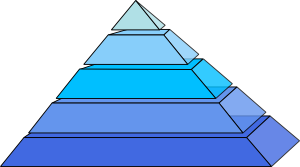
\includegraphics[width=1.1cm]{../Strukturfiler/FIGS/BluePyramid} & \begin{minipage}{\obsl}}{\end{minipage}\\ \end{tabular}\vspace{4mm}\newline}


% = Forudsætning = basis
\newenvironment{basis}{\begin{flushleft} \begin{itshape} }{\end{itshape} \end{flushleft}}


% = Opsummering =
\newenvironment{summary}{\clearpage\pagecolor{sumgul}\section{Opsummering}}{\newpage\pagecolor{white}}











% = Counter
\newcounter{opgavecount}[section]
\setcounter{opgavecount}{0}
\newcounter{spgcount}[opgavecount]
\setcounter{spgcount}{0}
\renewcommand{\thespgcount}{\alph{spgcount})}



% = EXERCISE = (DIVIDER)

\newcommand{\exercisebegin}[1][]{\bigskip\needspace{3\baselineskip}\refstepcounter{opgavecount}\titlegraphic{mingroen}\textcolor{mingroen}{\th{Opgave \theopgavecount \hspace*{1cm} #1}}\medskip\par}

% = QUIZEXERCISE = (DIVIDER)

\newcommand{\quizexercisebegin}[1][]{\bigskip\needspace{3\baselineskip}\refstepcounter{opgavecount}\titlegraphic{mingroen}\textcolor{mingroen}{\th{Quiz-Opgave \theopgavecount \hspace*{1cm} #1}}\medskip\par}

% = QUESTION =

\newenvironment{question}{\refstepcounter{spgcount}\begin{itemize}\item[\thespgcount]}{\end{itemize}\hspace*{\fill}}

% = VINK =

\newenvironment{vink}{\begin{tabular}{m{.9cm}<{\hspace*{2mm}}@{}|m{\obsl}@{}}\hspace*{-4pt}\raggedleft
\includegraphics[width=.9cm]{../Strukturfiler/FIGS/Think} & \begin{minipage}{\obsl}}{\end{minipage}\\ \end{tabular}\medskip\\}
	
% = FACIT =

\newenvironment{facit}{\begin{tabular}{m{.9cm}<{\hspace*{2mm}}@{}|m{\obsl}@{}}\hspace*{-4pt}\raggedleft
\includegraphics[width=.9cm]{../Strukturfiler/FIGS/Check} & \begin{minipage}{\obsl}}{\end{minipage}\\ \end{tabular}\medskip\\}








\newcommand{\afsnit}[1]{\bigskip\th{\titlegraphic{mingroen}\textcolor{mingroen}{#1}} \\ \rule[7pt]{.4\textwidth}{1pt} \vspace*{-2.5mm}\par}

% (DIVIDER):
\newcommand{\ugedagdatotitel}[4]{\pagebreak[4]\section{Semesteruge #1 -- #2 Dag \hspace*{1mm} (#3)} \vspace*{-4mm} \rule[5pt]{\textwidth}{1pt}\vspace*{-2.5mm} \begin{center}\large{\th{#4}}\end{center} \fancyhead[C]{\th{Semesteruge #1}}}

\newenvironment{skema}[1]{\definecolor{shadecolor}{rgb}{0.96,.98, 1.0} \setlength{\FrameSep}{6pt} \renewcommand{\FrameHeightAdjust}{10pt} \vspace*{-4pt}\begin{shaded} \begin{tabular}{#1}}{\end{tabular} \end{shaded} \vspace*{-7pt}}


% ========================

% MAKROER

%\newenvironment{matr}[1][]{\hspace*{-.8mm}\left[\hspace*{-1mm}\begin{array}{#1}}{\end{array}\hspace*{-1mm}\right]\hspace*{-.8mm}}
\newcommand{\bevisslut}{\begin{scriptsize} \begin{flushright} $ \blacksquare $ \end{flushright} \end{scriptsize}}

\newcommand{\tref}[2]{\hyperref[#1]{#2 \ref*{#1}}}
\newcommand{\thref}[2]{\hyperref[#1]{#2}}

\newcommand{\refA}[1]{\colorbox{yellow}{\ref{#1}}}
\newcommand{\hrefA}[2]{\colorbox{yellow}{\href{#1}{#2}}}
\newcommand{\trefA}[2]{\colorbox{yellow}{\hyperref[#1]{#2 \ref*{#1}}}}
\newcommand{\threfA}[2]{\colorbox{yellow}{\hyperref[#1]{#2}}}

\newenvironment{matr}[1]{\hspace*{-.8mm}\begin{bmatrix}\hspace*{-1mm}\begin{array}{#1}}{\end{array}\hspace*{-1mm}\end{bmatrix}\hspace*{-.8mm}}
\newcommand{\transp}{\hspace*{-.6mm}^{\top}}

\newcommand{\maengde}[2]{\left\lbrace \hspace*{-1mm} \begin{array}{c|c} #1 & #2 \end{array} \hspace*{-1mm} \right\rbrace}

\newenvironment{eqnalign}[1]{\setlength{\arraycolsep}{1.3pt}\begin{equation}\begin{array}{#1}}{\end{array}\end{equation}\par}
\newcommand{\eqnl}{\setlength{\arraycolsep}{1.3pt}}

\newcommand{\matind}[3]{{_\mathrm{#1}\mathbf{#2}_\mathrm{#3}}}
\newcommand{\vekind}[2]{{_\mathrm{#1}\mathbf{#2}}}
\newcommand{\jac}[2]{{\mathrm{Jacobi}_\mathbf{#1} (#2)}}
\newcommand{\diver}[2]{{\mathrm{div}\mathbf{#1} (#2)}}
\newcommand{\rot}[1]{{\mathbf{rot}\mathbf{(#1)}}}

\newcommand{\am}{\mathrm{am}}
\newcommand{\gm}{\mathrm{gm}}
\newcommand{\E}{\mathrm{E}}
\newcommand{\Span}{\mathrm{span}}
\newcommand{\mU}{\mathbf{U}}

\newcommand{\ms}{\medskip\\}
\newcommand{\bs}{\bigskip\\}

\newcommand{\mA}{\mathbf{A}}
\newcommand{\mB}{\mathbf{B}}
\newcommand{\mC}{\mathbf{C}}
\newcommand{\mD}{\mathbf{D}}
\newcommand{\mE}{\mathbf{E}}
\newcommand{\mF}{\mathbf{F}}
\newcommand{\mK}{\mathbf{K}}
\newcommand{\mI}{\mathbf{I}}
\newcommand{\mM}{\mathbf{M}}
\newcommand{\mN}{\mathbf{N}}
\newcommand{\mQ}{\mathbf{Q}}
\newcommand{\mT}{\mathbf{T}}
\newcommand{\mV}{\mathbf{V}}
\newcommand{\mW}{\mathbf{W}}
\newcommand{\mX}{\mathbf{X}}
\newcommand{\ma}{\mathbf{a}}
\newcommand{\mb}{\mathbf{b}}
\newcommand{\mc}{\mathbf{c}}
\newcommand{\md}{\mathbf{d}}
\newcommand{\me}{\mathbf{e}}
\newcommand{\mn}{\mathbf{n}}
\newcommand{\mr}{\mathbf{r}}
\newcommand{\mv}{\mathbf{v}}
\newcommand{\mw}{\mathbf{w}}
\newcommand{\mx}{\mathbf{x}}
\newcommand{\mxb}{\mathbf{x_{bet}}}
\newcommand{\my}{\mathbf{y}}
\newcommand{\mz}{\mathbf{z}}
\newcommand{\reel}{\mathbb{R}}
\newcommand{\mL}{\bm{\Lambda}} %Lambda-matrix
\newcommand{\mnul}{\bm{0}}
\newcommand{\trap}[1]{\mathrm{trap}(#1)}
\newcommand{\Det}{\operatorname{Det}}
\newcommand{\adj}{\operatorname{adj}}
\newcommand{\Ar}{\operatorname{Areal}}
\newcommand{\Vol}{\operatorname{Vol}}
\newcommand{\Rum}{\operatorname{Rum}}
\newcommand{\diag}{\operatorname{\bf{diag}}}
\newcommand{\bidiag}{\operatorname{\bf{bidiag}}}
\newcommand{\spanVec}[1]{\mathrm{span}\{#1\}}
\newcommand{\Div}{\operatorname{Div}}
\newcommand{\Rot}{\operatorname{\mathbf{Rot}}}

\newcommand{\Jac}{\operatorname{Jacobi}}
\newcommand{\Tan}{\operatorname{Tan}}
\newcommand{\Ort}{\operatorname{Ort}}
\newcommand{\Flux}{\operatorname{Flux}}
\newcommand{\Cmass}{\operatorname{Cm}}
\newcommand{\Imom}{\operatorname{Im}}
\newcommand{\Pmom}{\operatorname{Pm}}
\newcommand{\IS}{\operatorname{I}}
\newcommand{\IIS}{\operatorname{II}}
\newcommand{\IIIS}{\operatorname{III}}
\newcommand{\Le}{\operatorname{L}}
\newcommand{\app}{\operatorname{app}}
\newcommand{\M}{\operatorname{M}}
\newcommand{\re}{\mathrm{Re}}
\newcommand{\im}{\mathrm{Im}}

\newcommand{\compl}{\mathbb{C}} %de komplekse tal
\newcommand{\e}{\mathrm{e}} %eksponentialfunktionen. lodret 'e', og altså ikke kursiv ligesom andre bogstaver.





% Medialink: SCREEN: (QRcode) + thumbnail image + link på kodenummer (til qr.dtu.dk)
\newcommand{\onlinemedia}[3]{
	\begin{wrapfigure}{r}{3.2cm} 
		\vspace{-30pt} 
		\vspace{#1pt} 
		\begin{flushright} 
			\includegraphics[width=3cm]{qr/#2.png} 
			\tiny 
			\href{http://qr.dtu.dk/#2}{#2: #3}
			\normalsize  
		\end{flushright} 
		\vspace{-10pt} 
	\end{wrapfigure}
}
\newcommand{\onlinemediathumb}[3]{
	\begin{wrapfigure}{r}{3.2cm} 
		\vspace{-30pt} 
		\vspace{#1pt} 
		\begin{flushright} 
			\includegraphics[width=3cm]{qr/#2.png} 
			\includegraphics[width=3cm]{qr/#2_thumb.png} 
			\tiny 
			\href{http://qr.dtu.dk/#2}{#2: #3}
			\normalsize  
		\end{flushright} 
		\vspace{-10pt} 
	\end{wrapfigure}
}



% Index:
\usepackage{makeidx}
\makeindex
\newcommand\ind[2]{\index{#1}\textbf{\textit{\textcolor{black}{#2}}}}

% ###SERVER_EXCLUDE_BEGIN###
\externaldocument[NUID17-]{../../enoten/TN01-Talrum/Talrum}
\externaldocument[NUID1-]{../../enoten/TN02-Ligningssystemer/TNdriver}
\externaldocument[NUID2-]{../../enoten/TN03-Matricer_og_Matrixalgebra/Matricer_og_matrixalgebra}
\externaldocument[NUID3-]{../../enoten/TN04-Kvadratiske_matricer/TNdriver}
\externaldocument[NUID11-]{../../enoten/TN05-Determinanter/Determinanter}
\externaldocument[NUID12-]{../../enoten/TN06-GeometriskeVektorer/GeometriskeVektorer}
\externaldocument[NUID18-]{../../enoten/TN07-Vektorrum/VektorRum}
\externaldocument[NUID21-]{../../enoten/TN08-LinAfbildninger/LinAfbildninger}
\externaldocument[NUID23-]{../../enoten/TN09-Egenvaerdier_og_egenvektorer/TNdriver}
\externaldocument[NUID24-]{../../enoten/TN10-Diagonalisering_med_egenvektorer/TNdriver}
\externaldocument[NUID10-]{../../enoten/TN11-1.ordens_differentialligninger/TNdriver}
\externaldocument[NUID13-]{../../enoten/TN12-1.ordens_differentialligningssystemer/TNdriver}
\externaldocument[NUID14-]{../../enoten/TN13-2.ordens_differentialligninger/TNdriver}
\externaldocument[NUID27-]{../../enoten/TN14-Elemenataere_funktioner/Elementaere_Funktioner}
\externaldocument[NUID28-]{../../enoten/TN15-Funktioner2Variable/Funktioner_To_Variable}
\externaldocument[NUID29-]{../../enoten/TN16-Gradienter_og_Tangentplaner/Gradienter_og_Tangentplaner}
\externaldocument[NUID32-]{../../enoten/TN17-Taylor_formler/Taylor_Formler}
\externaldocument[NUID33-]{../../enoten/TN18-Taylor_2Var/Taylor_2Var}
\externaldocument[NUID34-]{../../enoten/TN19-SymMat/SymmetriskeMatricer}
\externaldocument[NUID35-]{../../enoten/TN20-KegleSnit/Keglesnit}
\externaldocument[NUID36-]{../../enoten/TN21-Riemann_Integral/Riemann_01}
\externaldocument[NUID37-]{../../enoten/TN22-Plan_Int/Plan_Int_01}
\externaldocument[NUID39-]{../../enoten/TN23-Flade_Int/Flade_Rum_Int_01}
\externaldocument[NUID40-]{../../enoten/TN24-Vektorfelter/Vektorfelter_01}
\externaldocument[NUID41-]{../../enoten/TN25-Flux/Flux_02}
\externaldocument[NUID42-]{../../enoten/TN26-Gauss/Gauss_01}
\externaldocument[NUID128-]{../../enoten/TN27-Stokes/Stokes_01}
\externaldocument[NUID43-]{../../enoten/TN29-KomplekseTal/KomplekseTal}

\externaldocument[NUID6-]{../../E-math-opgaver/Opgaver/opgU123}
\externaldocument[NUID19-]{../../E-math-opgaver/Opgaver/opgU45}
\externaldocument[NUID20-]{../../E-math-opgaver/Opgaver/opgU678}
\externaldocument[NUID25-]{../../E-math-opgaver/Opgaver/opgU910SD}
\externaldocument[NUID31-]{../../E-math-opgaver/OpgaverF11-U123/opgF123}
% \externaldocument[NUID9-]{../../E-math-opgaver/Opgaver/Dagsordner E10}
% ###SERVER_EXCLUDE_END###


% Begin document and set alternative chapter title:
\begin{document}
\renewcommand{\chaptername}{eNote}

\setcounter{chapter}{3} %SÆT DETTE TAL TIL 1 MINDRE END DET AKTUELLE TRANSFERNOTE-NUMMER!!

%%%%%%%%%%%%%%%%%%%%%%%%%%%%%%%%%%%%%%%%%%%%%
%%% HERFRA SKAL DU SKRIVE ELLER INDSÆTTE %%%%
%%% DEN FIL DU ØNSKER %%%%%%%%%%%%%%%%%%%%%%%
%%%%%%%%%%%%%%%%%%%%%%%%%%%%%%%%%%%%%%%%%%%%%

\chapter{Kvadratiske matricer} \label{tn4}

\begin{basis} 
I denne eNote undersøges grunlæggende egenskaber ved mængden af kvadratiske matricer herunder indførelse af en invers matrix for visse kvadratiske matricer. Det forudsættes at man kender til de basale matrixoperationer, se for eksempel \tref{NUID2-tn3}{eNote}.
\end{basis}

Kvadratiske matricer er ganske enkelt matricer, som har \textit{lige mange rækker og søjler}, så de er af typen $ n \times n $. Noten her vil introducere nogle af de grundlæggende operationer, der findes med kvadratiske matricer. \bs
En kvadratisk $ n \times n $ matrix $ \mA $ ser således ud:
\begin{equation}
\mA = \begin{matr}{cccc} a_{11} & a_{12} & \ldots & a_{1n} \\ a_{21} & a_{22} & \ldots & a_{2n} \\ \vdots & \vdots & & \vdots \\ a_{n1} & a_{n2} & \ldots & a_{nn} \end{matr}
\end{equation}
Elementer $ a_{11}, a_{22}, \ldots, a_{nn} $ siges at stå i \ind{hoveddiagonal}{hoveddiagonalen} eller bare \textit{diagonalen} i $ \mA $. \bs
En kvadratisk matrix $ \mD $, som kun har elementer forskellige fra nul i hoveddiagonalen, kaldes en \ind{diagonalmatrix}{diagonalmatrix}, og man kan betegne den $ \mD = \diag(a_{11},a_{22},\ldots,a_{nn}) $. \bs
En \ind{symmetrisk matrix}{symmetrisk matrix} $ \mA $ er en kvadratrisk matrix, som er lig sin egen transponerede, altså $ \mA = \mA\transp $. \bs
Den kvadratiske matrix, som har 1-taller i hoveddiagonalen og nuller ellers, kaldes for \ind{enhedsmatrix}{enhedsmatricen} uanset antallet af rækker og søjler. Enhedsmatricen betegnes med \ind{$ \mE $, enhedsmatrix}{$ \mE $}. Man har altså, at
\begin{equation}
\mE = \mE_{n \times n} = \begin{matr}{rrrr} 1 & 0 & \cdots & 0 \\ 0 & 1 & \cdots & 0 \\ \vdots & \vdots & \ddots & \vdots \\ 0 & 0 & \ldots & 1 \end{matr}
\end{equation}

\begin{aha}
I udenlandsk litteratur betegnes enhedsmatricen ofte med $ \mI $ (identity matrix).
\end{aha}

\begin{theorem}[Enhedsmatricen]
Enhedsmatricen $\mE$ i $\reel^{n\times n}$ er den eneste matrix i $\reel^{n\times n}$ som opfylder følgende sammenhænge:
\begin{equation}
\mA \mE = \mE \mA = \mA
\end{equation}
for en vilkårlig matrix $ \mA \in \reel^{n\times n}\,$.
\end{theorem}

\begin{bevis}
%Enhedsmatricen er den eneste matrix, hvor sammenhængene $ \mA \mE = \mE \mA = \mA $ gælder for en vilkårlig matrix $ \mA $. \bs 
Man kan forestille sig en anden matrix $ \mD $, hvor samme sammenhænge var gældende, altså at $ \mA \mD = \mD \mA = \mA $ for en vilkårligt matrix $ \mA $. Denne vilkårlige matrix kunne være enhedsmatricen, og sammenfatter man så de to ligninger får man: $ \mD = \mE \mD = \mD \mE = \mE $. \bs
Da $ \mE = \mD $, findes der altså ikke andre matricer end enhedsmatricen $ \mE $, der er neutralt element for matrixproduktet.
\end{bevis}

\begin{aha}
Enhedsmatricen kan betragtes som ''matricernes $1$-tal'': Ligesom man ikke ændrer ikke en skalar ved at gange den med $1$, ændrer man ikke en matrix ved at lave matrixproduktet af matricen med enhedsmatricen af samme type.
\end{aha}

Som det vil fremgå af det følgende, er det ofte ved brug af kvadratiske matricer afgørende om de har fuld rang eller ej. Derfor indfører vi nu særlige  begreber til at udtrykke dette.

\begin{definition}[Regulær og singulær matrix]

En kvadratisk matrix kaldes \ind{regulær matrix}{regulær}, hvis den har fuld rang, det vil sige at $ \rho(\mA_{n \times n}) = n $.\bs
En kvadratisk matrix kaldes \ind{singulær matrix}{singulær}, hvis den ikke har fuld rang, det vil sige at $ \rho(\mA_{n \times n}) < n $. 

\end{definition}

\section{Invers matrix}
%Det er ikke muligt at dividere med matricer, men enhedsmatricen kan hjælpe med at komme frem til en lignende operation. \bs
%At dividere med en skalar forskellig fra $0$ er det samme som at gange med dens reciprokke. Derfor kan vi koncentrere os om at finde den reciprokke, da matrixproduktet allerede er defineret.
Den reciprokke til en skalar $ a \neq 0 $ opfylder følgende ligning: $ a \cdot x = 1 $, hvor $ x $ er den reciprokke. Man kan omskrive det til, at $ x = a^{-1} $. Denne idé vil vi nu generalisere til kvadratiske matricer. Læg her mærke til, at man ikke kan bestemme den reciprokke til en skalar $a$, hvis $ a=0 $. En lignende undtagelse dukker op når vi generaliserer til kvadratiske matricer.\bs
Til at bestemme den ``reciprokke matrix'' til en matrix $ \mA $, kaldet den inverse matrix, opstilles en \textit{matrixligning} svarende til $ a \cdot x = 1 $ for en skalar:
\begin{equation}
\mA \mX = \mX \mA = \mE \label{tn4.lig.1}
\end{equation}
Den ubekendte $ \mX $ er en matrix. Hvis der findes en løsning $ \mX\,$,  betegnes den \ind{$ \mA^{-1} $, invers matrix}{$ \mA^{-1} $} og kaldes den \ind{invers matrix}{inverse matrix} til $ \mA $. Vi ønsker altså at finde en bestemt matrix kaldet $ \mA^{-1} $, som netop opfylder at matrixproduktet af $ \mA $ med den giver enhedsmatricen. \bs
Det er dog ikke alle kvadratiske matricer, som har en invers matrix. 
%, ligesom man ikke kan bestemme den reciprokke til $ a = 0 $.
 Det postuleres i følgende sætning.

\begin{theorem}[Invers matrix] \label{tn4.findesinvers}
En kvadratisk matrix $ \mA_{n \times n} $ har en invers matrix $ \mA^{-1} $, der opfylder $ \mA \mA^{-1} = \mA^{-1} \mA = \mE $, hvis og kun hvis $ \mA $ er regulær. \bs
Den inverse matrix bestemmes entydigt ved løsning af  matrixligningen $ \mA \mX = \mE $, hvor $ \mX $ er den ubekendte.
\end{theorem}



%En regulær matrix svarer altså til, at $ a \neq 0 $. \bs
I den følgende metode forklares, hvordan man løser den før beskrevne matrixligning \eqref{tn4.lig.1}, og derved finder den inverse, såfremt matricen er regulær.

\begin{method}[At bestemme den inverse matrix] \label{tn4.findinvers}
Man bestemmer den inverse matrix, betegnet $ \mA^{-1} $, til den regulære kvadratiske matrix $ \mA $ ved hjælp af \textit{matrixligningen}
\begin{equation}
\mA\mX = \mE.
\end{equation}
Ligningen løses med hensyn til den ubekendte $ \mX $ på følgende måde:
\begin{enumerate}
\item Totalmatricen $ \mT = \begin{matr}{c|c} \mA & \mE \end{matr} $ opstilles.
\item Ved sædvanlig GaussJordan-elimination bestemmes trappeformen af $ \mT $: $ \trap{\mT} $, hvor man i første omgang kan ignorere placeringen af den lodrette streg.
\item Ved eliminationen dannes til slut enhedsmatricen på venstre side af den lodrette streg, mens løsningen (den inverse til $ \mA $) kan aflæses på højre side: $ \trap{\mT} = \begin{matr}{c|c} \mE & \mX \end{matr} = \begin{matr}{c|c} \mE & \mA^{-1} \end{matr} $ .
\end{enumerate}
\end{method}

\begin{example}[Invers matrix] \label{tn4.invers}
Vi ønsker at finde den inverse matrix $ \mA^{-1} $ til matricen $ \mA $, som er givet således:
\begin{equation}
\mA = \begin{matr}{rrr} -16 & 9 & -10 \\ 9 & -5 & 6 \\ 2 & -1 & 1 \end{matr}
\end{equation}
Dette kan gøres ved hjælp af metode \ref{tn4.findinvers}. Først opstilles totalmatricen:
\begin{equation}
\mT = \begin{matr}{rrr|rrr} -16 & 9 & -10 & 1 & 0 & 0 \\ 9 & -5 & 6 & 0 & 1 & 0 \\ 2 & -1 & 1 & 0 & 0 & 1 \end{matr}
\end{equation}
Nu danner vi det ledende 1-tal i første række: Først rækkeoperationen $ R_1 + R_2 $ og derefter $ R_1 + 4 \cdot R_3 $. Det giver
\begin{equation}
\begin{matr}{rrr|rrr} -7 & 4 & -4 & 1 & 1 & 0 \\ 9 & -5 & 6 & 0 & 1 & 0 \\ 2 & -1 & 1 & 0 & 0 & 1 \end{matr} \quad \rightarrow \quad
\begin{matr}{rrr|rrr} 1 & 0 & 0 & 1 & 1 & 4 \\ 9 & -5 & 6 & 0 & 1 & 0 \\ 2 & -1 & 1 & 0 & 0 & 1 \end{matr}
\end{equation}
Så fjernes tallene i 1. søjle af 2. og 3. række: $ R_2 -9 \cdot R_1 $ og $ R_3 -2 \cdot R_1 $. Endvidere byttes 2. og 3. række: $ R_2 \leftrightarrow R_3 $. Vi får da
\begin{equation}
\begin{matr}{rrr|rrr} 1 & 0 & 0 & 1 & 1 & 4 \\ 0 & -5 & 6 & -9 & -8 & -36 \\ 0 & -1 & 1 & -2 & -2 & -7 \end{matr} \quad \rightarrow \quad
\begin{matr}{rrr|rrr} 1 & 0 & 0 & 1 & 1 & 4 \\ 0 & -1 & 1 & -2 & -2 & -7 \\ 0 & -5 & 6 & -9 & -8 & -36 \end{matr}
\end{equation}
Nu ændrer vi fortegnet på række 2: $ (-1) \cdot R_2 $ og derefter fjernes tallet i 2. søjle af 3. række: $ R_3 +5 \cdot R_2 $.
\begin{equation}
\begin{matr}{rrr|rrr} 1 & 0 & 0 & 1 & 1 & 4 \\ 0 & 1 & -1 & 2 & 2 & 7 \\ 0 & -5 & 6 & -9 & -8 & -36 \end{matr} \quad \rightarrow \quad
\begin{matr}{rrr|rrr} 1 & 0 & 0 & 1 & 1 & 4 \\ 0 & 1 & -1 & 2 & 2 & 7 \\ 0 & 0 & 1 & 1 & 2 & -1 \end{matr}
\end{equation}
Sidste skridt er da umiddelbar: $ R_2 + R_3 $:
\begin{equation}
\trap{\mT} = \begin{matr}{rrr|rrr} 1 & 0 & 0 & 1 & 1 & 4 \\ 0 & 1 & 0 & 3 & 4 & 6 \\ 0 & 0 & 1 & 1 & 2 & -1 \end{matr}
\end{equation}
Det ses, at $ \rho(\mA) = \rho(\mT) = 3 $, altså har $ \mA $ fuld rang, og derfor kan man aflæse den inverse til $ \mA $ på højresiden af den lodrette streg:
\begin{equation}
\mA^{-1} = \begin{matr}{rrr} 1 & 1 & 4 \\ 3 & 4 & 6 \\ 1 & 2 & -1 \end{matr}
\end{equation}

\begin{aha}
Læg mærke til, at venstresiden af totalmatricen er enhedsmatricen. Den er altså ''flyttet'' fra højre til venstre side af lighedstegnene (den lodrette streg).
\end{aha}
Til sidst kontrollerer vi, om $ \mA^{-1} $ som forventet opfylder $ \mA\mA^{-1} = \mE $ og $ \mA^{-1}\mA = \mE $:
\begin{equation}
\begin{aligned}
&\mA\mA^{-1} = \begin{matr}{rrr} -16 & 9 & -10 \\ 9 & -5 & 6 \\ 2 & -1 & 1 \end{matr} \begin{matr}{rrr} 1 & 1 & 4 \\ 3 & 4 & 6 \\ 1 & 2 & -1 \end{matr} \\
&= \begin{matr}{c c c} \begin{matr}{rrr} -16 & 9 & -10 \\ 9 & -5 & 6 \\ 2 & -1 & 1 \end{matr} \begin{matr}{r} 1 \\ 3 \\ 1 \end{matr} & \begin{matr}{rrr} -16 & 9 & -10 \\ 9 & -5 & 6 \\ 2 & -1 & 1 \end{matr} \begin{matr}{r} 1 \\ 4 \\ 2 \end{matr} & \begin{matr}{rrr} -16 & 9 & -10 \\ 9 & -5 & 6 \\ 2 & -1 & 1 \end{matr} \begin{matr}{r} 4 \\ 6 \\ -1 \end{matr} \end{matr} \\
&= \begin{matr}{ccc} -16+27-10 & -16+36-20 & -64+54+10 \\ 9-15+6 & 9-20+12 & 36-30-6 \\ 2-3+1 & 2-4+2 & 8-6-1 \end{matr} = 
\begin{matr}{ccc} 1 & 0 & 0 \\ 0 & 1 & 0 \\ 0 & 0 & 1 \end{matr} = \mE
\end{aligned}
\end{equation}
Det passer! Ved brug af samme fremgangsmåde ses, at også $ \mA^{-1}\mA = \mE $ passer.
\end{example}

Som man kan se i næste eksempel, så kan man bruge den inverse til at løse matrixligninger med kvadratiske matricer. I matrixligninger kan man nemlig også \textit{bytte rundt på led} og \textit{gange med skalare} for at isolere den ubekendte ligesom i almindelige lineære ligninger med skalarer. Ydermere kan man \textit{gange igennem} med matricer -- dette kan enten gøres fra højre eller venstre på alle leddene i ligningen, hvilket giver forskellige resultater.

\begin{example}[Matrixligning] \label{tn4.matligning}
Vi ønsker at løse matrixligningen
\begin{equation}
\mA\mX = \mB - \mC\mX
\end{equation}
hvor
\begin{equation}
\mA = \begin{matr}{rrr} -4 & 2 & -1 \\ 9 & 5 & -5 \\ 2 & 0 & 7 \end{matr} \quad , \quad \mB = \begin{matr}{rrr} 0 & 1 & 0 \\ 8 & -12 & 5 \\ 5 & 0 & 0 \end{matr} \quad \mathrm{og} \quad \mC = \begin{matr}{rrr} -12 & 7 & -9 \\ 0 & -10 & 11 \\ 0 & -1 & -6 \end{matr}
\end{equation}
Først reduceres ligningen så meget som muligt, se eventuelt \tref{NUID2-tn3.regneregler2}{sætning}, uden at bruge værdierne:
\begin{equation}
\mA\mX = \mB - \mC\mX \, \Leftrightarrow \, \mA\mX + \mC\mX = \mB - \mC\mX + \mC\mX \, \Leftrightarrow \, (\mA + \mC)\mX = \mB
\end{equation}
Da $ \mX $ er den ubekendte, vil vi prøve at isolere den helt. Er $ (\mA + \mC) $ en regulær matrix, kan man gange med den inverse til $ (\mA + \mC) $ fra venstre på begge sider af lighedstegnet. Altså:
\begin{equation}
(\mA + \mC)^{-1} (\mA + \mC)\mX = (\mA + \mC)^{-1} \mB \, \Leftrightarrow \, \mE\mX = \mX = (\mA + \mC)^{-1} \mB \, ,
\end{equation}
fordi $ (\mA + \mC)^{-1} (\mA + \mC) = \mE $ ifølge definitionen på inverse matricer. Vi laver nu matrixsummen $ \mA + \mC $ og ser om matricen er regulær:
\begin{equation}
\mA + \mC = \begin{matr}{rrr} -4 & 2 & -1 \\ 9 & 5 & -5 \\ 2 & 0 & 7 \end{matr} + \begin{matr}{rrr} -12 & 7 & -9 \\ 0 & -10 & 11 \\ 0 & -1 & -6 \end{matr} = \begin{matr}{rrr} -16 & 9 & -10 \\ 9 & -5 & 6 \\ 2 & -1 & 1 \end{matr}
\end{equation}
Den inverse til denne matrix er allerede bestemt i eksempel \ref{tn4.invers}, og den del af proceduren springes derfor over. $ \mX $ kan da bestemmes:
\begin{equation}
\begin{aligned}
\mX &= (\mA + \mC)^{-1} \mB = {\begin{matr}{rrr} -16 & 9 & -10 \\ 9 & -5 & 6 \\ 2 & -1 & 1 \end{matr}}^{-1} \begin{matr}{rrr} 0 & 1 & 0 \\ 8 & -12 & 5 \\ 5 & 0 & 0 \end{matr} \\
&= \begin{matr}{rrr} 1 & 1 & 4 \\ 3 & 4 & 6 \\ 1 & 2 & -1 \end{matr} \begin{matr}{rrr} 0 & 1 & 0 \\ 8 & -12 & 5 \\ 5 & 0 & 0 \end{matr} = \begin{matr}{rrr} 28 & -11 & 5 \\ 62 & -45 & 20 \\ 11 & -23 & 10 \end{matr}
\end{aligned}
\end{equation}
\end{example}

For videre undersøgelse af invertibilitet af den transponerede eller inverse af en regulær matrix samt  invertibilitet af produktet af to eller flere regulære matricer får vi brug for følgende hjælpesætning. Anføres uden bevis.

\begin{lemma}[Arvet regularitet]
$1.$ Hvis $\mA$ er en regulær kvadratisk matrix, er såvel $\mA\transp$ som $\mA^{-1}$ også regulære.\bs
$2.$ Produktet $\mA\,\mB$ af to kvadratiske matricer er regulært hvis og kun hvis både $\mA$ og $\mB$ er regulære.
\end{lemma}

Vi kan herefter opstille regneregler for inverse matricer.

\begin{theorem}[Regneregler ved invers matrix] \label{tn4.regner}

For de regulære kvadratiske matricer $ \mA, \mB $ og $ \mC $ gælder der følgende regneregler:
\begin{enumerate}
\item Den inverse til den inverse af en matrix er lig matricen selv:
\begin{equation}
(\mA^{-1})^{-1} = \mA \label{tn4.regner2}
\end{equation}
\item Den transponerede til en invers matrix er det samme som den inverse transponerede matrix: 
\begin{equation}
(\mA\transp)^{-1} = (\mA^{-1})\transp \label{tn4.regner3}
\end{equation}
$ \mA\transp $ er regulær, hvis og kun hvis $ \mA $ er regulær.
\item I matrixligninger kan man gange igennem med den inverse til en matrix. Dette kan gøres enten fra højre eller venstre på begge sider af lighedstegnet:
\begin{equation}
\mA \mX = \mB \Leftrightarrow \mX = \mA^{-1} \mB \quad \mathrm{og} \quad \mX \mC = \mD \Leftrightarrow \mX = \mD \mC^{-1} \label{tn4.regner1}
\end{equation}
\item Den inverse til et matrixprodukt af to matricer er lig produktet af de tilsvarende inverse matricer i omvendt rækkefølge:
\begin{equation}
(\mA \mB)^{-1} = \mB^{-1} \mA^{-1}
\end{equation}
%$ \mA\mB $ er regulær, hvis og kun hvis både $ \mA $ og $ \mB $ er regulære.
\end{enumerate}
\end{theorem}

Alle regnereglerne i sætning \ref{tn4.regner} bevises nemt ved at ''gøre prøve''.\bs
%\begin{aha}
%Den første regneregel \eqref{tn4.regner2} i sætning \ref{tn4.regner} bygger på noget, som indtil videre ikke er konstateret: Den inverse til en (regulær) matrix er også regulær! Det vil sige, at det også er muligt at finde den inverse til denne matrix. Regnereglen påpeger så, at den inverse til den inverse til en matrix er lig matricen selv. \bs
%På samme måde er den transponerede af en regulær matrix også regulær, hvilket udnyttes i den anden regneregel, \eqref{tn4.regner3}.
%\end{aha}
Herunder afprøves en af reglerne i et eksempel. Regnereglen i ligning \eqref{tn4.regner1} er allerede blevet brugt i eksempel \ref{tn4.matligning}. 

\begin{example}[Eftervisning af regneregel ved invers matrix]
Der er givet to kvadratiske matricer
\begin{equation}
\mA = \begin{matr}{rr} 2 & 4 \\ 6 & 10 \end{matr} \quad \mathrm{og} \quad \mB = \begin{matr}{rr} 1 & 1 \\ 2 & 3 \end{matr}
\end{equation}
Vi ønsker at afprøve den sidste regneregel i sætning \ref{tn4.regner}, nemlig at $ (\mA \mB)^{-1} = \mB^{-1} \mA^{-1} $. Først bestemmes $ \mA^{-1} $ og $ \mB^{-1} $ ved hjælp af metode \ref{tn4.findinvers}.
\begin{equation}
\begin{matr}{c|c} \mA & \mE \end{matr} = \begin{matr}{rr|rr} 2 & 4 & 1 & 0 \\ 6 & 10 & 0 & 1 \end{matr} \rightarrow \begin{matr}{rr|rr} 1 & 2 & \tfrac{1}{2} & 0 \\ 0 & -2 & -3 & 1 \end{matr} \rightarrow \begin{matr}{rr|rr} 1 & 0 & -\tfrac{5}{2} & 1 \\ 0 & 1 & \tfrac{3}{2} & -\tfrac{1}{2} \end{matr}
\end{equation}
På samme måde med $ \mB $:
\begin{equation}
\begin{matr}{c|c} \mB & \mE \end{matr} = \begin{matr}{rr|rr} 1 & 1 & 1 & 0 \\ 2 & 3 & 0 & 1 \end{matr} \rightarrow \begin{matr}{rr|rr} 1 & 1 & 1 & 0 \\ 0 & 1 & -2 & 1 \end{matr} \rightarrow \begin{matr}{rr|rr} 1 & 0 & 3 & -1 \\ 0 & 1 & -2 & 1 \end{matr}
\end{equation}
Da det er lykkedes at få enhedsmatricen på venstresiden af stregen i begge tilfælde, har vi nu at
\begin{equation}
\mA^{-1} = \begin{matr}{rr} -\tfrac{5}{2} & 1 \\ \tfrac{3}{2} & -\tfrac{1}{2} \end{matr} \quad \mathrm{og} \quad
\mB^{-1} = \begin{matr}{rr} 3 & -1 \\ -2 & 1 \end{matr}
\end{equation}
$ \mB^{-1}\mA^{-1} $ bestemmes:
\begin{equation} \label{tn4.lig.2}
\mB^{-1}\mA^{-1} = \begin{matr}{cc} \begin{matr}{rr} 3 & -1 \\ -2 & 1 \end{matr} \begin{matr}{r} -\tfrac{5}{2} \\ \tfrac{3}{2} \end{matr} & \begin{matr}{rr} 3 & -1 \\ -2 & 1 \end{matr} \begin{matr}{r} 1 \\ -\tfrac{1}{2} \end{matr} \end{matr} = 
\begin{matr}{rr} -9 & \tfrac{7}{2} \\ \tfrac{13}{2} & -\tfrac{5}{2} \end{matr}
\end{equation}
På den anden side af lighedstegnet i regnereglen haves i første omgang $ \mA\mB $:
\begin{equation} 
\mA\mB = \begin{matr}{cc} \begin{matr}{rr} 2 & 4 \\ 6 & 10 \end{matr}\begin{matr}{r} 1 \\ 2 \end{matr} & \begin{matr}{rr} 2 & 4 \\ 6 & 10 \end{matr} \begin{matr}{r} 1 \\ 3 \end{matr}\end{matr} = \begin{matr}{rr} 10 & 14 \\ 26 & 36 \end{matr}
\end{equation}
Nu bestemmes den inverse til $ \mA\mB $:
\begin{equation}
\begin{matr}{c|c} \mA\mB & \mE \end{matr} = \begin{matr}{rr|rr} 10 & 14 & 1 & 0 \\ 26 & 36 & 0 & 1 \end{matr} \rightarrow \begin{matr}{rr|rr} 1 & \tfrac{7}{5} & \tfrac{1}{10} & 0 \\ 0 & -\frac{2}{5} & -\frac{13}{5} & 1 \end{matr} \rightarrow 
\begin{matr}{rr|rr} 1 & 0 & -9 & \frac{7}{2} \\ 0 & 1 & \frac{13}{2} & -\frac{5}{2} \end{matr}
\end{equation}
Vi har altså, at
\begin{equation} \label{tn4.lig.3}
(\mA\mB)^{-1} = \begin{matr}{rr} -9 & \frac{7}{2} \\ \frac{13}{2} & -\frac{5}{2} \end{matr} \, ,
\end{equation}
Sammenlignes ligning \eqref{tn4.lig.2} og \eqref{tn4.lig.3} ses, at der er fuldstændig lighed: $ (\mA \mB)^{-1} = \mB^{-1} \mA^{-1} $.
\end{example}

\begin{exercise}[Invers matrix]
Givet er matricerne
\begin{equation}
\mA = \begin{matr}{rr} 0 & 1 \\ 1 & 0 \\ 2 & 3 \end{matr} \quad \mathrm{og} \quad \mB = \begin{matr}{rrr} 3 & 2 & 1 \\ 0 & 1 & 2 \end{matr}
\end{equation}
%%%%%FORSLAG TIL OPGAVER !!!
\renewcommand{\labelenumi}{\alph{enumi})}
%%%%
\begin{enumerate}
\item Bestem $ (\mB\mA)^{-1} $.
\item Vis, at $ \mA\mB $ ikke er regulær, og man derfor ikke kan bestemme $ (\mA\mB)^{-1} $.
\end{enumerate}
\end{exercise}

\begin{exercise}[Invers matrix]
Givet er matricerne
\begin{equation}
\mA = \begin{matr}{rr} 2 & 3 \\ 1 & 1 \end{matr} \, , \quad \mB = \begin{matr}{rr} 1 & 0 \\ 4 & 1 \end{matr} \, , \quad \mC = \begin{matr}{rr} -1 & 3 \\ 1 & -2 \end{matr} \quad \mathrm{og} \quad \mD = \begin{matr}{rr} 1 & 0 \\ -4 & 1 \end{matr}
\end{equation}
%%%%%FORSLAG TIL OPGAVER !!!
\renewcommand{\labelenumi}{\alph{enumi})}
%%%%
\begin{enumerate}
\item Udregn $ \mA\mC $, $ \mB\mD $ og $ \mD\mC $.
\item Angiv, hvis det er muligt, $ \mA^{-1} $, $ \mB^{-1} $ og $ (\mA\mB)^{-1} $. 
\item Er det muligt at sige, om $ (\mA\mB)^{-1} $ findes efter at have prøvet at bestemme $ \mA^{-1} $ og $ \mB^{-1} $? Hvis ja, hvordan?
\end{enumerate}
\end{exercise}

\section{Potenser af matricer}

Vi har nu set, hvordan den inverse til en regulær matrix bestemmes, og vi siger, at den har potensen $ -1 $. Tilsvarende defineres her vilkårlige heltallige \ind{potens af kvadratisk matrix}{potenser af kvadratiske matricer}.

\begin{definition}[Potens af matrix] \label{tn4.defpotens}
For en vilkårlig kvadratisk matrix $ \mA $ defineres følgende naturlige potenser:
\begin{equation}
\mA^0 = \mE \quad \mathrm{og} \quad \mA^n = \overbrace{\mA \mA \cdots \mA}^{n~\mathrm{gange}} \, , \, \mathrm{for}~n \in \mathbb{N}
\end{equation}
For en vilkårlig \textbf{regulær} kvadratisk matrix $ \mB $ defineres yderligere de negative potenser:
\begin{equation}
\mB^{-n} = (\mB^{-1})^n = \overbrace{\mB^{-1} \mB^{-1} \cdots \mB^{-1}}^{n~\mathrm{gange}} \, , \, \mathrm{for}~n \in \mathbb{N}
\end{equation}
\end{definition}

Som følge af definitionen på potenserne, kan nogle regneregler opskrives.

\begin{theorem}[Regneregler for potenser af matricer] \label{tn4.defpotensregne}
For en vilkårlig kvadratisk matrix $ \mA $ og to vilkårlige ikke negative heltal $ a $ og $ b $ gælder følgende potensregneregler
\begin{equation}
\mA^a \mA^b = \mA^{a+b} \quad \mathrm{og} \quad (\mA^a)^b = \mA^{ab}
\end{equation}
Er $ \mA $ regulær, gælder disse regneregler også for negative heltal $ a $ og $ b $.
\end{theorem}

Herunder er et eksempel på to (simple) matricer, som har nogle pudsige egenskaber. Egenskaberne er \textit{ikke} typiske for matricer, og der findes slet ikke nogle tilsvarende skalarer. 

\begin{example}[To pudsige matricer mht. potenser]
Givet er matricerne
\begin{equation}
\mA = \begin{matr}{rr} 1 & 0 \\ 2 & -1 \end{matr} \quad \mathrm{og} \quad \mB = \begin{matr}{rr} 2 & 1 \\ -4 & -2 \end{matr}
\end{equation}
Med hjælp fra både definition \ref{tn4.defpotens} og sætning \ref{tn4.defpotensregne} laves følgende udregninger. $ \mA^2 $ bestemmes:
\begin{equation}
\mA^2 = \mA\mA = \begin{matr}{rr} 1 & 0 \\ 2 & -1 \end{matr} \begin{matr}{rr} 1 & 0 \\ 2 & -1 \end{matr} = \begin{matr}{rr} 1 & 0 \\ 0 & 1 \end{matr} = \mE
\end{equation}
Ifølge tilføjelsen til den fjerde regneregel i sætning \ref{tn4.regner} er $ \mA $ da regulær, og desuden er $ \mA = \mA^{-1} $. Det giver
\begin{equation}
\begin{array}{ll}
\; \vdots & \; \vdots \\
\mA^{-3} = (\mA\mA^2)^{-1} = \mA^{-1} = \mA \hspace*{1cm} & \mA^{-2} = (\mA^2)^{-1} = \mE \\
\mA^{-1} = \mA & \mA^0 = \mE \\
\mA^1 = \mA & \mA^2 = \mE \\
\; \vdots & \; \vdots \\
\end{array}
\end{equation}
Alle ulige potenser af $ \mA $ giver altså $ \mA $ selv, mens de lige potenser giver enhedsmatricen:
\begin{equation}
\mA^{2n} = \mE \; \mathrm{~og~} \; \mA^{2n+1} = \mA \; \mathrm{~for~} \; n \in \mathbb{Z}
\end{equation}
$ \mB^2 $ udregnes:
\begin{equation}
\mB^2 = \begin{matr}{rr} 2 & 1 \\ -4 & -2 \end{matr}\begin{matr}{rr} 2 & 1 \\ -4 & -2 \end{matr} = \begin{matr}{rr} 0 & 0 \\ 0 & 0 \end{matr} = \mnul
\end{equation}
Ifølge samme regneregel er $ \mB $ singulær. Man har da, at
\begin{equation}
\mB^0 = \mE \, , \, \mB^1 = \mB \, , \, \mB^2 = \mnul \, , \, \mB^n = \mnul \; \mathrm{~for~} \; n \geq 2
\end{equation}
\end{example}

\begin{summary}
\begin{itemize}
\item Kvadratiske matricer er matricer med lige mange rækker og søjler.
\item Enhedsmatricen $ \mE $ er en kvadratisk matrix med ettaller i diagonalen og nuller ellers:
\begin{equation}
\mE = \mE_{n \times n} = \begin{matr}{rrrr} 1 & 0 & \cdots & 0 \\ 0 & 1 & \cdots & 0 \\ \vdots & \vdots & \ddots & \vdots \\ 0 & 0 & \ldots & 1 \end{matr}
\end{equation}
\item Hvis en kvadratisk matrix har fuld rang, kaldes den regulær, ellers kaldes den singulær.
\item En kvadratisk matrix, som kun har tal forskellige fra nul i diagonalen, kaldes en diagonalmatrix.
\item En kvadratisk matrix, som er lig sin egen transponerede, kaldes en symmetrisk matrix.
\item Til en regulær matrix $ \mA $ findes den inverse, betegnet $ \mA^{-1} $, der opfylder at
\begin{equation}
\mA\mA^{-1} = \mA^{-1}\mA = \mE
\end{equation}
Den inverse kan bestemmes ved hjælp af metode \ref{tn4.findinvers}.
\item Der findes regneregler med kvadratiske og inverse matricer, se sætning \ref{tn4.regner}.
\item Potenser af kvadratiske matricer er defineret, se definition \ref{tn4.defpotens}. Dertil findes også nogle regneregler.
\item Inverse matricer bruges for eksempel i forbindelse med \textit{basisskifte} og \textit{egenværdiproblemet}. Desuden defineres \textit{determinanten} af en kvadratisk matrix i \tref{NUID11-tn5}{eNote}.
\end{itemize}
\end{summary}

%%%%%%%%%%%%%%%%%%%%%%%%%%%%%%%%%%%%%%%%%%%%%
%%% HER SKAL DU STOPPE MED AT SKRIVE %%%%%%%%
%%%%%%%%%%%%%%%%%%%%%%%%%%%%%%%%%%%%%%%%%%%%%


\end{document} 